\chapter{Формализация многокритериальной оптимизационной задачи, методы сведения к однокритериальной, решение с использованием Optimization Toolbox системы Matlab.}
\section{Постановка задачи}
\subsection{Индивидуальное задание}
\textbf{Задача 2}\\
Фабрика производит два вида изделий, А и Б. Продажа изделий осуществляется на внутреннем рынке и также экспортируется в другие страны. Стоимость изделия А на внутреннем рынке \$30, а на внешнем - \$45, стоимость изделия Б на внутреннем рынке \$20, а на внешнем - \$21.

Для изготовления изделий используются два вида станков. Для изготовления 1 единицы изделия А необходима работа первого станка в течении 1 часа и второго – в течение 2 часов, а для изготовления 1 единицы изделия Б необходима работы первого станка в течение 5 часов и второго в течение 7 часов. Ресурс времени непрерывной работы 1 станка 18 часов, а 2 – 20 часов. 

Изучение рынка сбыта показало, что спрос на изделие А никогда не превышает 5000 изделий в сутки, а на изделие Б - 9000. 

Какое количество изделий каждого вида надо производить в  данных условиях для внутреннего и для внешнего рынков, чтобы доход от реализации продукции на внутреннем рынке был максимальным?  Какое количество изделий каждого вида надо производить, чтобы минимизировать время использования станков при  условии использования не менее 80\% ресурса непрерывной работы каждого станка? Какое количество изделий каждого вида надо производить в  данных условиях, чтобы доход от реализации продукции на экспорт был максимальным?

\subsection{Пункты расчетного задания}
\begin{enumerate}
\item Осуществить переход от многокритериальной задачи к однокритериальной с использованием следующих подходов:
\begin{itemize}
\item Выделение главного критерия;
\item Свертка критериев (аддитивная и мультипликативная);
\item Максимин или минимакс (он же метод максиминной свертки);
\item Метод последовательных уступок;
\item fgoalattain;
\item Ведение метрики в пространстве критериев.
\end{itemize}
\item Решить задачу стохастического программирования для одной из однокритериальных задач, превратив детерминированное ограничение в вероятностное по схеме
\end{enumerate}
\begin{equation}
P(\sum_{j=1}^{n} a_{ij}x_j-b_i\leq 0)\geq a_i
\end{equation}
Менять $a_i$ в следующем диапазоне $0,1\leq a_i\leq 0,9$
 
Считать случайной величиной $b_i$ или элементы ${a_{ij} i}$-й строки матрицы $A{a_{ij}}$ (по выбору).
%\pmb{$$}

\section{Математическая модель задачи многокритериальной оптимизации}
\begin{itemize}
\item $x_{11}$ – количество изделий А на внутреннем рынке;
\item $x_{12}$ – количество изделий A на внешнем рынке;
\item $x_{21}$ – количество изделий Б на внутреннем рынке;
\item $x_{22}$ – количество изделий Б на внешнем рынке.
\end{itemize}
\textbf{Первый критерий}. Максимизация дохода на внутреннем рынке
\begin{equation}
f_1 (x_{11}, x_{21})=30*x_{11}+20*x_{21} \rightarrow max 
\end{equation}
\textbf{Второй критерий}. Минимизация использования станков

\begin{equation}
\begin{split}
f_2 (x_{11}, x_{12}, x_{21}, x_{22})=\\ &
\left(x_{11}+x_{12})+2*(x_{11}+x_{12})+5*(x_{21}+x_{22})+7*(x_{21}+x_{22}\right)=\\ & 
3*\left(x_{11}+x_{12})+12*(x_{21}+x_{22}\right) \rightarrow min
\end{split}
\end{equation}
\textbf{Третий критерий}. Максимизация дохода на внешнем рынке
\begin{equation}
f_3 (x_{12}, x_{22})= 45*x_{12}+21*x_{22} \rightarrow max
\end{equation}
\textbf{Примечание: решений, с ограничением на использование не менее 80\% ресурса непрерывной работы станков, найти не удалось. Поэтому данное ограничение было снижено до 70\%.}\\
\textbf{Также часы были переведены в минуты.}\\\\
\textbf{Ограничения:}\\
Для станков первого типа
\begin{equation}
1*(x_{11}+x_{12})+5*(x_{21}+x_{22})\leq 18*60
\end{equation}
\begin{equation} \label{limit:1}
1*(x_{11}+x_{12})+5*(x_{21}+x_{22})\geq (18*60)*0.7
\end{equation}
Для станков второго типа
\begin{equation}
2*(x_{11}+x_{12})+7*(x_{21}+x_{22})\leq 20*60
\end{equation}
\begin{equation} \label{limit:2}
2*(x_{11}+x_{12})+7*(x_{21}+x_{22})\geq (20*60)*0.7
\end{equation}
Ограничения по количеству изделий
\begin{equation}
\begin{cases}
x_{11}+x_{12}\leq 5000\\
x_{21}+x_{22}\leq 9000
\end{cases}
\end{equation}
С учетом требований пакета MATLAB к постановке задач оптимизации, необходимо представить целевые функции как поиск минимумов, а ограничения записать в виде $g(x) \leq 0$. Изменим ограничения \ref{limit:1} и \ref{limit:2}, а также введем новые функции, где $z_1=-f_1, z_3=-f_3$. В итоге получим:
\begin{equation}
z_1 (x_{11}, x_{21})=-(30*x_{11}+20*x_{21}) \rightarrow min 
\end{equation}
\begin{equation}
z_3 (x_{12}, x_{22})= -(45*x_{12}+21*x_{22}) \rightarrow min
\end{equation}
\textbf{Ограничения:}
\begin{equation}
\begin{cases}
1*(x_{11}+x_{12})+5*(x_{21}+x_{22})\leq 18*60\\
-1*(x_{11}+x_{12})-5*(x_{21}+x_{22})\leq -(18*60)*0.7\\
2*(x_{11}+x_{12})+7*(x_{21}+x_{22})\leq 20*60\\
-2*(x_{11}+x_{12})-7*(x_{21}+x_{22})\leq -(20*60)*0.7\\
x_{11}+x_{12}\leq 5000\\
x_{21}+x_{22}\leq 9000
\end{cases}
\end{equation}
\subsection{Поиск оптимумов частных критериев}
Найдем оптимумы каждой из целевых функций независимо от других. Для этого необходимо решить три задачи однокритериальной оптимизации: для $z_1, f_2, z_3$ при тех же ограничениях на $x_{11}, x_{12}, x_{21}, x_{22}$ что имеют место для задачи многокритериальной оптимизации.

Для решение данной задачи, был использован MATLAB, код с общими параметрами приведен в приложении 1.

\begin{lstlisting}[language={matlab}, caption={Поиск оптимумов частных критериев}, label={lst:1}]
%% Поиск оптимумов частных критериев
startingPoint = lb;
[x, z1_opt] = fmincon(z1, startingPoint, A, b, Aeq, beq, lb, ub)
[x, f2_opt] = fmincon(f2, startingPoint, A, b, Aeq, beq, lb, ub)
[x, z3_opt] = fmincon(z3, startingPoint, A, b, Aeq, beq, lb, ub)
\end{lstlisting}

\begin{lstlisting}[language={matlab}, caption={Результаты выполнения листинга \ref{lst:1}}]
x =
  236.0000
    0.0000
  104.0000
    0.0000
z1_opt =
  -9.1600e+03

x =
    0.0000
    0.0000
   75.6000
   75.6000
f2_opt =
   1.8144e+03

x =
  0.0000
  236.0000
  0.0000
  104.0000

z3_opt =
  -1.2804e+04

\end{lstlisting}
Таким образом, были получены следующие оптимальные значения:
\begin{equation}
z_1^{min}=-9160, f_2^{min}=1814.4, z_3^{min}=-12804
\end{equation}
Откуда следует:
\begin{enumerate}
\item $f_1^{max} = 9160\$$ - максимальный доход на внутреннем рынке;
\begin{itemize}
\item $x_{11}$ - 236;
\item $x_{21}$ - 104.
\end{itemize}
\item $f_2^{min}=1814.4$ часов - общее время использования первого и второго станка;
\begin{itemize}
\item $x_{21}$ - 75.6;
\item $x_{22}$ - 75.6;
\item Примечание: значение в 151.2(75.6+75.6) изделий Б, упирается в нижнюю границу(756 часов(70\%)) первого станка.
\end{itemize}
\item $f_3^{max}=12804\$$ - максимальный доход на внешнем рынке.
\begin{itemize}
\item $x_{12}$ - 236;
\item $x_{22}$ - 104.
\end{itemize}
\end{enumerate}
Также были посчитаны значения прочих критериев при оптимуме каждого критерия.

\tabulinesep = 1mm
\begin{longtabu} to \textwidth {|X[ c , m ] |X[c , m ] | X[ c , m ]|X[ c , m ]|X[ c , m ]|X[ c , m ]|X[ c , m ]|}\firsthline\hline
\textbf{$x_{11}$}&\textbf{$x_{12}$}&\textbf{$x_{21}$}&\textbf{$x_{22}$}&\textbf{$f_{1}$}&\textbf{$f_{2}$}&\textbf{$f_{3}$}\\ \hline \endfirsthead
\multicolumn{7}{|c|}{Оптимум $f_1$}\\ \hline
236&0&104&0&9160&1956&0\\ \hline
\multicolumn{7}{|c|}{Оптимум $f_2$}\\ \hline
0&0&75.6&75.6&1512&1814.4&1587.6\\ \hline
\multicolumn{7}{|c|}{Оптимум $f_3$}\\ \hline
0&236&0&104&0&1956&12804\\ \hline

\caption{Оптимумы критериев и значения функций}
\end{longtabu}
Как видно из таблицы, оптимум первого или третьего критерия означает 0 велечину другого критерия.


\section{Переход от многокритериальной задачи к однокритериальной}
\subsection{Выделение главного критерия}
%Один из критериев - главный - имеет существенно более высокий приоритет, чем все остальные. Пусть главный критерий - первый, тогда для двух оставшихся критериев составим ограничения.


Один из критериев - главный - имеет существенно более высокий приоритет, чем все остальные, но по остальным критериям вариант тоже не должен быть слишком плох. Пусть главный критерий - первый, следовательно, для оставшихся целевых функций необходимо указать нижние границы. Предположим, что общее время изготовления продукции ($f_2$) должно быть не более 1950 часов, а доход на внешнем рынке должен быть больше 1000\$. Таким образом, к задаче добавляются еще 2 ограничения:
\begin{equation}
3*(x_{11}+x_{12})+12*(x_{21}+x_{22})\leq 1950 
\end{equation}
\begin{equation}
45*x_{12}+21*x_{22}\geq 1000
\end{equation}
В соответствии с изменениями скрипт был дополнен ограничениями(Код приведен в приложении 2).

После выполнения программы были получены следующие результаты:
\begin{lstlisting}[language={matlab}, caption={Результаты выполнения листинга \ref{lst:2}}]
x =

  203.7778
   22.2222
  106.0000
    0.0000


f_val =

  -8.2333e+03
\end{lstlisting}
Таким образом было получено значение в 8233.3\$, что составляет 89\% от оптимума. 
Время использования станков - 1950 часов(упор в ограничение), доход на внешнем рынке - 1000\$(упор в ограничение).
\begin{itemize}
\item $f_1$ - 8233.3\$ (89.9\% от оптимума);
\item $f_2$ - 1950 часов (на 7.4\% больше оптимума);
\item $f_3$ - 1000\$ (7.8\% от оптимума);
\item 9 233.3\$ - общий доход.
\end{itemize}
Столь низкий процент от оптимума у $f_3$ объясняется тем, что большая часть изделий продавалась на внутренний рынок, а не на внешний.


\subsection{Свертка критериев}
\subsubsection{Аддитивная свертка критериев}
Для использования метода аддитивной свертки необходимо выполнить нормировку критериев, с тем чтобы сделать их значения соизмеримыми, а единицы измерения – безразмерными. Выполним нормировку следующим образом:



\begin{equation}
\overline{z_1} = \frac{z_1}{|z_1^{min}|} =-\frac{30*x_{11}+20*x_{21}}{9160} = -\frac{3*x_{11}+2*x_{21}}{916} 
\end{equation}

\begin{equation}
\overline{f_2} = \frac{f_2}{|f_2^{min}|} = \frac{3*(x_{11}+x_{12})+12*(x_{21}+x_{22})}{1814.4}  = \frac{x_{11}+x_{12}+4*(x_{21}+x_{22})}{604.8}  
\end{equation}

\begin{equation}
\overline{z_3} = \frac{z_3}{|z_3^{min}|} = \frac{-45*x_{12}+21*x_{22}}{12804} =   \frac{-15*x_{12}+7*x_{22}}{4266.8}
\end{equation}

Формула аддитивной свертки имеет вид:
\begin{equation}
F(x) = \sum_{i=1}^{r}\lambda_i f_i(x), 0<\lambda_i<1, \sum_i^{}\lambda_i=1,
\end{equation}
где $f_i(x)$ - критерии оптимальности, $r$ – их общее число, а $\lambda_i$ - параметры важности. Примем $\lambda_1=0.4, \lambda_2=0.2, \lambda_3=0.4$. Для этого добавим к листингу \ref{lst:1} следующий код:
\begin{lstlisting}[language={matlab}, caption={Аддитивная свертка}, label={lst:add}]
% Аддитивная свертка
z1_norm = @(N) z1(N)/abs(z1_opt);
f2_norm = @(N) f2(N)/abs(f2_opt);
z3_norm = @(N) z3(N)/abs(z3_opt);
f = @(N) 0.4*z1_norm(N) +0.2*f2_norm(N) + 0.4*z3_norm(N);
A = [1,1,5,5;
    -1,-1,-5,-5;
    2,2,7,7;
    -2,-2,-7,-7;
    1,1,0,0;
    0,0,1,1
    3,3,12,12;
    0,-45,0,-21];
b = [Tmax1; -Tmin1; Tmax2; -Tmin2;  5000; 9000; 1950; -1000];

[N, f_opt] = fmincon(f, startingPoint, A, b, Aeq, beq, lb, ub)
\end{lstlisting}
\begin{lstlisting}[language={matlab}, caption={Результаты выполнения листинга \ref{lst:add}}]
N =
    0.0009
  225.9990
  105.9997
    0.0004

f_opt =
   -0.1953
   
>> f1(N)
ans =
   2.1200e+03

>> f2(N)
ans =
   1.9500e+03

>> f3(N)
ans =
   1.0170e+04
\end{lstlisting}
Метод аддитивной свертки позволил получить решение:
\begin{itemize}
\item $f_1$ - 2120\$ (23.1\% от оптимума);
\item $f_2$ - 1950 часов (на 7.4\% больше оптимума);
\item $f_3$ - 10170\$ (79.4\% от оптимума);
\item 12 290\$ - общий доход.
\end{itemize}
\subsubsection{Мультипликативная свертка критериев}
Формула мультипликативной свертки имеет вид:
\begin{equation}
F(x) = \prod_{i=1}^{r}f_i(x)^{\lambda_i}
\end{equation}
где $f_i(x)$ - критерии оптимальности, $r$ - их общее число, а $\lambda_i$ - показатели важности. Примем $\lambda_1=0.4, \lambda_2=0.2, \lambda_3=0.4$. Данные значения были выбраны из соображения того что доход более важен чем минимизация времени станков. А также что доход на внутреннем и внешнем рынке одинаково важны.  Нормировка уже была произведена в аддитивной свертки, в итоге получим следующую задачу однокритериальной оптимизации:
\begin{equation}
f = \overline{z_1}^{0.4}*\overline{f_2}^{0.2}*\overline{z_3}^{0.4}
\end{equation}
Для этого добавим к листингу \ref{lst:1} следующий код:
\begin{lstlisting}[language={matlab}, caption={Мультипликативная свертка}, label={lst:mult}]
% Мультипликативная свертка
startingPoint = lb;
z1_norm = @(N) z1(N)/abs(z1_opt);
f2_norm = @(N) f2(N)/abs(f2_opt);
z3_norm = @(N) z3(N)/abs(z3_opt);
f = @(N) (-(f1(N)/9160)^0.4)*((f2(N)/1814.4)^0.2)*((f3(N)/12804)^0.4)
A = [1,1,5,5;
    -1,-1,-5,-5;
    2,2,7,7;
    -2,-2,-7,-7;
    1,1,0,0;
    0,0,1,1
    3,3,12,12;
    0,-45,0,-21];
b = [Tmax1; -Tmin1; Tmax2; -Tmin2;  5000; 9000; 1950; -1000];

[N, f_opt] = fmincon(f, startingPoint, A, b, Aeq, beq, lb, ub)
\end{lstlisting}
\begin{lstlisting}[language={matlab}, caption={Результаты выполнения листинга \ref{lst:mult}}]
N =
   77.6665
  148.3330
  105.9988
    0.0014

f_opt =
   -0.5858

>> f1(N)
ans =
   4.4500e+03

>> f2(N)
ans =
   1.9500e+03

>> f3(N)
ans =
   6.6750e+03
\end{lstlisting}
Метод мультипликативной свертки позволил получить решение:
\begin{itemize}
\item $f_1$ - 4450\$ (48.6\% от оптимума);
\item $f_2$ - 1950 часов (на 7.4\% больше оптимума);
\item $f_3$ - 6675\$ (52.1\% от оптимума);
\item 11 125\$ - общий доход.
\end{itemize}
Мультипликативная свертка позволила получить более компромиссное решение для $f_1$  и $f_3$, однако больший общий доход позволила получить аддитивная свертка.

\subsection{Минимакс (максимин)}
Максиминную свертку представим в следующем виде: $C_i(a)= \text{min } w_i C_i(a)$

Решение $a^*$ является наилучшим, если для всех $a$ выполняется условие $C(a^*) \geq C(a)$, или $a^* = \text{arg max } C(a) = \text{arg max min } w_i C_i (a)$.

Для реализации максиминной свертки необходимо в fminimax передавать функции обратные целевым (функция funminmax). Так как оцениваемые показатели разновелики, необходимо нормировать критерии. Что было произведено ранее.

Решение задачи представлено как скрипт в среде Matlab, для этого листинг \ref{lst:0} был дополнен:
\begin{lstlisting}[language={matlab}, caption={Минимакс (максимин)}, label={lst:minmax}]
%Минимакс - максимин
startingPoint = lb;
[x, f] = fminimax (@funminmax , startingPoint, A , b, Aeq, beq, lb, ub )

function f = funminmax (X)
f(1) = -(30*X(1) - 20*X(3))/9160;
f(2) = -(3*(X(1)+X(2))+12*(X(3)+X(4)))/1814.4;
f(3) = -(45*X(2) - 21*X(4))/12804;
end
\end{lstlisting}
\begin{lstlisting}[language={matlab}, caption={Результаты выполнения листинга \ref{lst:minmax}}]
x =

  123.4525
  112.5475
   46.9046
   57.0954

f =
   -0.3019   -1.0780   -0.3019

>> f1(x)
ans =
   4.6417e+03

>> f2(x)
ans =
        1956

>> f3(x)
ans =
   6.2636e+03
\end{lstlisting}
Метод минимакс (максимин) позволил получить решение:
\begin{itemize}
\item $f_1$ - 4641.7\$ (50.6\% от оптимума);
\item $f_2$ - 1956 часов (на 7.8\% больше оптимума);
\item $f_3$ - 6263.6\$ (48.9\% от оптимума);
\item 10905.3\$ - общий доход.
\end{itemize}
Процентное соотношение первого и второго критерия относительно оптимума примерно равное, второй критерий по сути игнорируется.

\subsection{Метод последовательных уступок}
Для решения данной задачи была выбрана уступка = 10\%. 	Предположим, что критерии пронумерованы в следующем порядке важности:
\begin{center}
$z_1>f_2>z_3$
\end{center} 
Для первого критерия уже решена задача поиска оптимального значения в п 1.2.1. То есть:
\begin{center}
$9160 * 0.9 = 8 244$
\end{center}
То ограничения критерия выглядит следующим образом:
\begin{center}
$-30*x_{11}-20*x_{21}\leq -8244$
\end{center}


Запишем ограничения в скрипт
\begin{lstlisting}[language={matlab}, caption={Последовательные уступки}]
...
% Функциональные ограничения
A = [1,1,5,5;
    -1,-1,-5,-5;
    2,2,7,7;
    -2,-2,-7,-7;
    1,1,0,0;
    0,0,1,1;
    -30,0,-20,0];
b = [Tmax1; -Tmin1; Tmax2; -Tmin2;  5000; 9000; -8244];

...

[x, z3_opt] = fmincon(z3, startingPoint, A, b, Aeq, beq, lb, ub)
\end{lstlisting}
\begin{lstlisting}[language={matlab}, caption={Результат выполнения}]
x =
  205.4667
   30.5333
  104.0000
    0.0000

z3_opt =
  -1.3740e+03
  
>> f1(x)
ans =
   8.2440e+03
\end{lstlisting}
Как и ожидалось при минимизации функции $z_3$ учитывалось и ограничения для $z_1$, что существенное уменьшило результат для $z_3$.

В соответствии с полученным значением введем ограничение для второго критерия.

\begin{center}
$1374 * 0.9 = 1236.6$
\end{center}
Ограничения критерия выглядит следующим образом:
\begin{center}
$-45*x_{12}-21*x_{22}\leq -1236.6$
\end{center}
Запишем ограничения в скрипт
\begin{lstlisting}[language={matlab}, caption={Последовательные уступки}]
...
% Функциональные ограничения
A = [1,1,5,5;
    -1,-1,-5,-5;
    2,2,7,7;
    -2,-2,-7,-7;
    1,1,0,0;
    0,0,1,1;
    -30,0,-20,0;
    0,-45,0,-21];
b = [Tmax1; -Tmin1; Tmax2; -Tmin2;  5000; 9000; -8244; -1236.6];

...

[x, z3_opt] = fmincon(z3, startingPoint, A, b, Aeq, beq, lb, ub)
\end{lstlisting}
\begin{lstlisting}[language={matlab}, caption={Результат выполнения}]
x =
  204.9969
   27.4800
  104.7046
    0.0000

f2_opt =
   1.9539e+03
  
>> f1(x)
ans =
   8.2440e+03
   
>> f3(x)
ans =
   1.2366e+03
\end{lstlisting}

Итоговые результаты:
\begin{itemize}
\item $f_1$ - 8244\$ (90\% от оптимума);
\item $f_2$ - 1953.9 часов (на 7.6\% больше оптимума);
\item $f_3$ - 1236.6\$ (9.6\% от оптимума);
\item 9 480.6\$ - общий доход.
\end{itemize}
По результатам видно, что за счет последовательности, при оптимизации каждого следующего критерия учитываются и уступка предыдущих критериев.

\subsection{Метод достижения цели (fgoalattain)}
Fgoalattain решает задачу достижения цели, которая является одной из формулировок
задач для векторной оптимизации.
x = fgoalattain(fun, $x_0$, goal, weight, ...):
\begin{itemize}
\item fun – целевая функция,
\item $x_0$ – начальные значения,
\item goal – целевые значения,
\item weight – веса.
\end{itemize}
Пусть goal = ($z_1^{min}, f_2^{min}, z_3^{min}$), w = ($|z_1^{min}|, |f_2^{min}|, |z_3^{min}|$). Тогда скрипт для решения задачи будет выглядеть следующим образом:
\begin{lstlisting}[language={matlab}, caption={Метод достижения цели}]
...
%% fgoalattain
f = @(N) [z1(N), f2(N), z3(N)];
goal = [z1_opt, f2_opt, z3_opt];
w = abs(goal);
A = [1,1,5,5;
    -1,-1,-5,-5;
    2,2,7,7;
    -2,-2,-7,-7;
    1,1,0,0;
    0,0,1,1];
b = [Tmax1; -Tmin1; Tmax2; -Tmin2;  5000; 9000];
lb = [0; 0; 0; 0];
ub = [5000; 5000; 9000; 9000];
startingPoint = lb;

[N, f_opt, af] = fgoalattain(f, startingPoint, goal, w, A, b, Aeq, beq, lb, ub)
\end{lstlisting}
\begin{lstlisting}[language={matlab}, caption={Результат выполнения}]
N =
  115.2789
  120.7211
   56.8321
   47.1679


f_opt =
   1.0e+03 *
   -4.5950    1.9560   -6.4230

af =
    0.4984
\end{lstlisting}
Значение переменной af, говорит о том, что полученное решение на 49.8\% хуже цели. 

Итоговые результаты:
\begin{itemize}
\item $f_1$ - 4595\$ (50.2\% от оптимума);
\item $f_2$ - 1956 часов (на 7.8\% больше оптимума);
\item $f_3$ - 6423\$ (50.2\% от оптимума);
\item 11 018\$ - общий доход.
\end{itemize}
Оба критерия $f_1$ и $f_3$ составляют одинаковую долю от своих оптимальных значений, в то время как второй критерий был проигнорирован, отдавая больший приоритет двум другим критериям.

\subsection{Введение метрики в пространстве критериев}
Для перехода к однокритериальной задаче оптимизации методом введения метрики в пространстве целевых функций необходимо определить координаты «идеальной» точки $a=(f_1^*, f_2^*, ..., f_r^*)$,  где $f_i = min f_i(x)$. Эти значения
уже были получены в п. 1.2.1, и поэтому:
\begin{center}
$a = (-9160, 1814.4, -12804)$
\end{center}
Введем в пространстве критериев метрику в виде евклидова расстояния:
\begin{equation}
p(y, a) = [\sum_{i=1}^r(a_i-y_i)^2]^{\frac{1}{2}} 
\end{equation}
Тогда за целевую функцию (обобщенный критерий), с учётом необходимости нормировки, можно взять выражение:
\begin{equation}
f=\sum_{i=1}^r(\frac{a_i-f_i}{f_i^*})^2=\sum_{i=1}^r(1-\frac{f_i}{f_i^*})^2
\end{equation}
Таким образом, получаем следующую задачу оптимизации:
\begin{equation}
f=(1-\frac{z_1}{z_1^{min}})^2+(1-\frac{f_2}{f_2^{min}})^2+(1-\frac{z_3}{z_3^{min}})^2
\end{equation}


\begin{lstlisting}[language={matlab}, caption={Метод достижения цели}]
...
% Параметрические ограничения
lb = [0; 0; 0; 0];
ub = [5000; 5000; 9000; 9000];

%% Поиск оптимумов частных критериев
startingPoint = lb;
[x, z1_opt] = fmincon(z1, startingPoint, A, b, Aeq, beq, lb, ub)
[x, f2_opt] = fmincon(f2, startingPoint, A, b, Aeq, beq, lb, ub)
[x, z3_opt] = fmincon(z3, startingPoint, A, b, Aeq, beq, lb, ub)

%% Введение метрики в пространстве критериев
f = @(N) (1-z1(N)/z1_opt)^2+(1-f2(N)/f2_opt)^2+(1-z3(N)/z3_opt)^2;
[N, f_opt] = fmincon(f, startingPoint, A, b, Aeq, beq, lb, ub)
\end{lstlisting}
\begin{lstlisting}[language={matlab}, caption={Результат выполнения}]
N =
   83.7126
  152.2874
  103.9999
    0.0001

f_opt =
    0.4709

>> f1(N)
ans =
   4.5914e+03

>> f2(N)
ans =
   1.9560e+03

>> f3(N)
ans =
   6.8529e+03
\end{lstlisting}
Итоговые результаты:
\begin{itemize}
\item $f_1$ - 4591.4\$ (50.1\% от оптимума);
\item $f_2$ - 1956 часов (на 7.8\% больше оптимума);
\item $f_3$ - 6852.9\$ (53.5\% от оптимума);
\item 11 444.3\$ - общий доход.
\end{itemize}

\section{Оценка Парето-оптимальности полученных решений}
Для того чтобы уменьшить количество альтернатив, среди которых лицо, принимающее решение (ЛПР), должно сделать выбор, можно выделить множество Парето среди всех полученных решений. Для этого была составлена таблица и построен график.


Столбец \textbf{SUM} означает общий доход с внешнего и внутреннего рынка, то есть $f_1+f_3$.
\tabulinesep = 1mm
\begin{longtabu} to \textwidth {|X[3, c , m ] |X[c , m ] | X[ c , m ]|X[ c , m ]|X[ c , m ]|X[ c , m ]|X[ c , m ]|X[ c , m ]|X[1.5, c , m ]|}\firsthline\hline
\textbf{Метод перехода к однокритериальной задаче}&\textbf{$x_{11}$}&\textbf{$x_{12}$}&\textbf{$x_{21}$}&\textbf{$x_{22}$}&\textbf{$f_1$}&\textbf{$f_2$}&\textbf{$f_3$}&\textbf{SUM}\\ \hline \endfirsthead
А. Выделение главного критерия&203.8&22.2&106&0&8233.3&1950&1000&9233.3\\ \hline
Б1. Аддитивная свертка&0&226&106&0&2120&1950&10170&12290\\ \hline
Б2. Мультипликативная свертка&77.7&148.3&106&0&4450&1950&6675&11125\\ \hline
В. Минимакс&123.45&112.55&46.9&57.1&4641.7&1956&6263.6&10905.3\\ \hline
Г. Метод последовательных уступок &205&27.5&105&0&8244&1953.9&1236.6&9480.6\\ \hline
Д. Метод достижения цели (fgoalattain) &115.3&120.7&56.8&47.2&4595&1956&6423&11018\\ \hline
Е. Введение метрики в пространстве критериев&83.7&152.3&104&0&4591.4&1956&6852.9&11444.3\\ \hline
\end{longtabu}
\begin{figure}[H]
	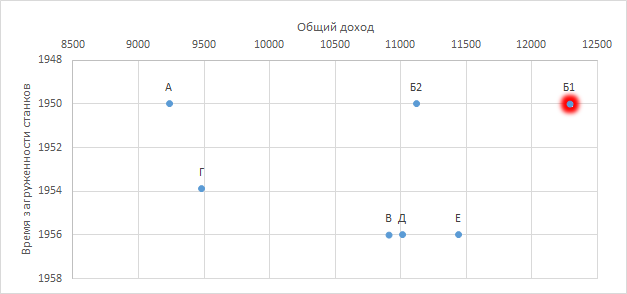
\includegraphics[width=\textwidth]{img/1}
	\caption{Оценки от полученных решений на плоскости критериев: красным выделено множество Парето}
\end{figure}  
Парето-оптимальными являются только решение Б1. С точки зрения ЛПР оно также является лучшим, так как позволяет достичь максимального дохода.

\section{Решение задачи стохастического программирования}
Рассмотрим задачу стохастического программирования на основе задачи однокритериальной оптимизации, которая была получена из исходной методом введения метрики в пространстве критериев (п. 1.3.6).

Преобразуем третье ограничение системы:
\begin{center}
$2x_{11}+2x_{12}+7*x_{21}+7*x_{22} \leq 1200$
\end{center}

 в вероятностное, тогда:
\begin{center}
$P(\alpha_{11}x_{11}+\alpha_{12}x_{12}+\alpha_{21}x_{21}+\alpha_{22}x_{22} \leq 1200)\geq \alpha$
\end{center}
где все $a_{ij}$ нормально распределены и имеют следующие математические ожидания и дисперсии:
\begin{center}
$M(\alpha_{11})=2, M(\alpha_{12})=2, M(\alpha_{21})=7, M(\alpha_{22})=7$
$D(\alpha_{11})=1, D(\alpha_{12})=1, D(\alpha_{21})=3.5, D(\alpha_{22})=3.5$
\end{center}
Где СКО равно половине математического ожидания. По таблице функции распределения стандартного нормального закона  находим $K_a (0.1\leq \alpha\leq 0.9)$
\begin{center}
$K_{0.1}=-1.2816, K_{0.2}=-0.8416, K_{0.3}=-0.5244, K_{0.4}=-0.2533, K_{0.5}=0$
$K_{0.6}=0.2533, K_{0.7}=0.5244, K_{0.8}=0.8416, K_{0.9}=1.2816$
\end{center}
Таким образом, вероятностное ограничение становится эквивалентно детерминированному неравенству:	
\begin{equation}
2x_{11}+2x_{12}+7*x_{21}+7*x_{22}+K_{\alpha}*\sqrt{x_{11}^2+x_{12}^2+3.5*x_{21}^2+3.5*x_{22}^2} \leq 1200
\end{equation}



Решение задачи представлено как скрипт в программе Matlab, код представлен в приложении 3.

\begin{lstlisting}[language={matlab}, caption={Результат выполнения}]
alpha = 0.1, X_11 = 271.4401, X_12 = 278.9110, x_21 = 41.1291, x_22 =  0.001, f1 = 8965.78, f2 = 2145, f3 = 12551.01
alpha = 0.2, X_11 = 271.4492, X_12 = 278.9046, x_21 = 41.1151, x_22 =  0.014, f1 = 8965.78, f2 = 2145, f3 = 12551.01
alpha = 0.3, X_11 = 271.4494, X_12 = 278.9048, x_21 = 41.1172, x_22 =  0.012, f1 = 8965.83, f2 = 2145, f3 = 12550.97
alpha = 0.4, X_11 = 155.5649, X_12 = 205.9867, x_21 = 78.8894, x_22 =  0.000, f1 = 6244.73, f2 = 2031, f3 = 9269.41
alpha = 0.5, X_11 = 83.7126, X_12 = 152.2874, x_21 = 103.9999, x_22 =  0.000, f1 = 4591.37, f2 = 1956, f3 = 6852.93
alpha = 0.6, X_11 = 63.7924, X_12 = 88.9527, x_21 = 74.5707, x_22 = 46.080, f1 = 3405.19, f2 = 1906, f3 = 4970.56
alpha = 0.7, X_11 = 27.7783, X_12 = 43.1165, x_21 = 73.8482, x_22 = 63.173, f1 = 2310.31, f2 = 1857, f3 = 3266.87
alpha = 0.8, X_11 = 0.0000, X_12 = 0.0000, x_21 = 74.3433, x_22 = 74.343, f1 = 1486.87, f2 = 1784, f3 = 1561.21
alpha = 0.9, X_11 = 0.0000, X_12 = 0.0000, x_21 = 70.9449, x_22 = 70.990, f1 = 1418.90, f2 = 1703, f3 = 1490.78 
Для детерминированных ограничений:
X_11 = 83.7126, X_12 = 152.2874, x_21 = 103.9999, x_22 =  0.000, f1 = 4591.37, f2 = 1956, f3 = 6852.93
\end{lstlisting}

\tabulinesep = 1mm
\begin{longtabu} to \textwidth {|X[ c , m ] |X[c , m ] | X[ c , m ]|X[ c , m ]|X[ c , m ]|X[ c , m ]|X[ c , m ]|X[ c , m ]|}\firsthline\hline
\textbf{$\alpha$}&\textbf{$x_{11}$}&\textbf{$x_{12}$}&\textbf{$x_{21}$}&\textbf{$x_{22}$}&\textbf{$f_1$}&\textbf{$f_2$}&\textbf{$f_3$}\\ \hline \endfirsthead
0.1&271.4401&278.9110&41.1291& 0.001&8965.78&2145&12551.01\\ \hline
0.2&271.4492&278.9046&41.1151& 0.014&8965.78&2145&12551.01\\ \hline
0.3&271.4494&278.9048&41.1172& 0.012&8965.83&2145&12550.97\\ \hline
0.4&155.5649&205.9867&78.8894& 0.000&6244.73&2031&9269.41\\ \hline
0.5&83.7126&152.2874&103.9999& 0.000&4591.37&1956&6852.93\\ \hline
0.6&63.7924&88.9527&74.5707&46.080&3405.19&1906&4970.56\\ \hline
0.7&27.7783&43.1165&73.8482&63.173&2310.31&1857&3266.87\\ \hline
0.8&0.0000&0.0000&74.3433&74.343&1486.87&1784&1561.21\\ \hline
0.9&0.0000&0.0000&70.9449&70.990&1418.90&1703&1490.78\\ \hline
\multicolumn{8}{|c|}{Решение задачи при детерминированных ограничениях}\\ \hline
-&83.7126&152.2874&103.9999& 0.000&4591.37&1956&6852.93\\ \hline
\end{longtabu}
Задача чувствительна к выбранному ограничению, т.к. для различных K получились разные результаты. 

Увеличение доверительной вероятности $\alpha$ приводит к ухудшению оценок получаемых решений по первому и второму критерию. При $\alpha = 0.5, K_{\alpha} = 0$в случае чего получается решение, совпадающее с решением задачи с детерминированными ограничениями. 

При $\alpha < 0.5$ квантиль приобретает отрицательное значение. За счет чего ограничения \textbf{ослабевают}(их выполнение становится менее важным), и например решение при $\alpha = 0.1$ практические совпадает с оптимум для первого и второго критерия одновременно, чего не удалось добиться в каких-либо методах оптимизации.

А при $\alpha > 0.5$ ограничения становяться более \textbf{жесткими}, что уменьшает общий доход.
